\documentclass[a4paper,11pt]{report}
%\documentclass{foils}

\usepackage{geometry,graphicx}
\usepackage{verbatim}
\usepackage{url}
\usepackage{html}
\usepackage{fancybox}
\usepackage{fancyhdr}
\usepackage{framed}
\usepackage{color}
\usepackage{multirow}

\usepackage{lingmacros}  % included with GenI
\usepackage{covington}   % included with GenI

% ----------------------------------------
\newcommand{\jargon}{\textbf}
\newcommand{\natlang}{\textit}
\newcommand{\semexpr}{\texttt}
\newcommand{\tautree}[1] {$\tau_{#1}$}
\newcommand{\koweytree}{\texttt}
\long\def\ignore#1{}

\newcommand{\fnparam}{\texttt}
\newcommand{\fnref}[1]{\textit{#1} (page \pageref{fn:#1})}
\newcommand{\fnreflite}[1]{\textit{#1}}
\newcommand{\fnlabel}[1]{\paragraph{#1}\label{fn:#1}}

\newcommand{\tuple}[1]{\langle #1 \rangle}
\setcounter{chapter}{-1}
\setcounter{secnumdepth}{3}
% ----------------------------------------

\geometry{verbose,tmargin=40mm,bmargin=40mm,lmargin=25mm,rmargin=25mm}
%\input{lambdaTeX}

\pagestyle{fancyplain} 
\lfoot{Geni source code}
\cfoot{\thepage}
\rfoot{}

%\setlength\parindent{0pt}
\setlength{\fboxsep}{0.1pt}

\renewcommand\FrameHeightAdjust{1pt}


\newenvironment{framedcode}% using default \FrameCommand
  {\MakeFramed {\advance\hsize-\width \FrameRestore}}%
  {\endMakeFramed}

\newenvironment{code}% using default \FrameCommand
  {\VerbatimEnvironment
   \footnotesize
   %\begin{framedcode}
   \begin{Verbatim}
  }%
  {\end{Verbatim} 
   %\end{framedcode}
   \normalsize }

%\lstloadlanguages{Haskell} 
%\lstnewenvironment{code} 
%    {\lstset{}% 
%      \csname lst@SetFirstLabel\endcsname} 
%    {\csname lst@SaveFirstLabel\endcsname} 
%    \lstset{ 
%      basicstyle=\small\ttfamily, 
%      flexiblecolumns=false, 
%      basewidth={0.5em,0.45em}, 
%      literate={-}{{$-$}}1 {+}{{$+$}}1 {/}{{$/$}}1 {*}{{$*$}}1 {=}{{$=$}}1 
%               {>}{{$>$}}1 {<}{{$<$}}1 {\\}{{$\lambda$}}1 
%               {->}{{$\rightarrow$}}2 {>=}{{$\geq$}}2 {<-}{{$\leftarrow$}}2 
%               {<=}{{$\leq$}}2 {=>}{{$\Rightarrow$}}2 {\ .}{{$\circ$}}2 
%               {>>}{{>>}}2 {>>=}{{>>=}}2 
%    } 

\begin{document}
\title{Literate Geni}
\author{Langue et Dialogue\\LORIA}

\maketitle
\tableofcontents

% -------------------------------------------------------------------------
% Overview 
% -------------------------------------------------------------------------

\chapter*{License}

GenI surface realiser\\
Copyright \copyright 2005 Carlos Areces and Eric Kow

\bigskip

This program is free software; you can redistribute it and/or
modify it under the terms of the GNU General Public License
as published by the Free Software Foundation; either version 2
of the License, or (at your option) any later version.

\bigskip

This program is distributed in the hope that it will be useful,
but WITHOUT ANY WARRANTY; without even the implied warranty of
MERCHANTABILITY or FITNESS FOR A PARTICULAR PURPOSE.  See the
GNU General Public License for more details.

\bigskip

You should have received a copy of the GNU General Public License
along with this program; if not, write to the Free Software
Foundation, Inc., 59 Temple Place - Suite 330, Boston, MA  02111-1307, USA.

\chapter{Overview}

\begin{figure}[h]
\begin{center}
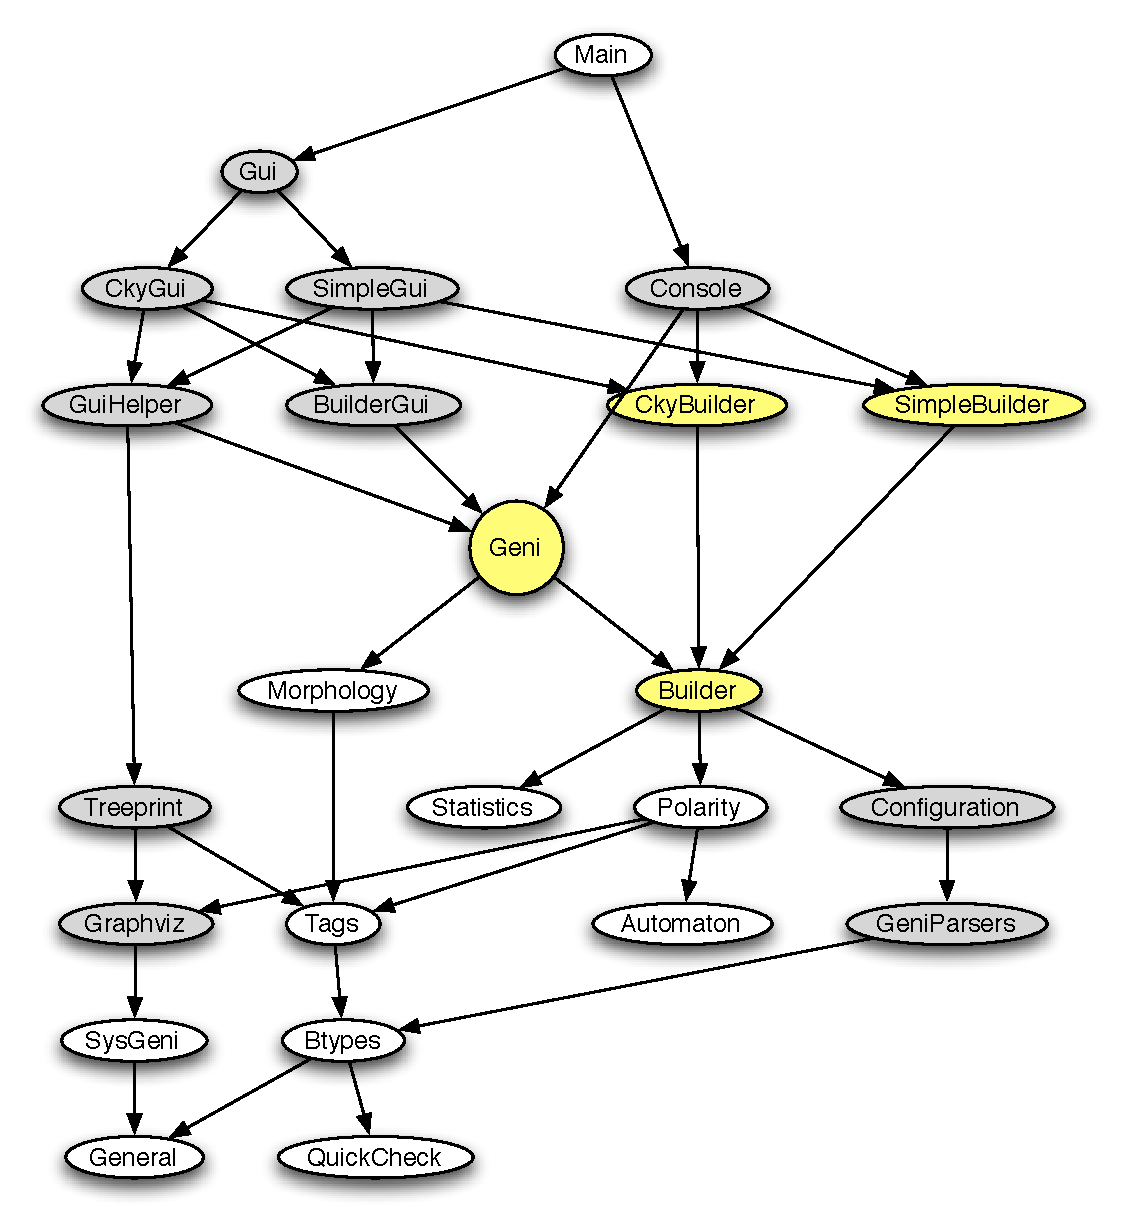
\includegraphics[scale=0.5]{images/genidep}
\caption{Transitive reduction of module dependencies}
\end{center}
\end{figure}

This document contains the source code to the GenI generator 
partly adapted to a literate programming style.  

\section{Core files}

Geni.lhs and Mstate.lhs perform the candidate selection and generation.
They will tend make heavy use of the modules Btypes.lhs and Tags.lhs, in
which we try to encapsulate some basic or generic operations into the
files.

\begin{description}
 \item[Main.lhs] - determines which user interface to run 
 \item[Geni.lhs] - parses and formats data for the generator 
 \item[Builder.lhs] - a chart generator   
 \item[SimpleBuilder.lhs] - the chart generator itself (note: substitution,
 adjunction, FS unification are done here, not in Tags.lhs)
 \item[CkyBuilder.lhs] - CKY version of the chart generator
 \item[Btypes.lhs] - basic data types and operations
 \item[Tags.lhs] - TAG specific data types
 \item[Automaton.lhs] - NFA  
\end{description}

\section{Enhancements}

This portion is for optimisations and other optional features of the
generator.
In addition to the modules below, chapter \ref{chp:other_optimisations}
will point you to ones which could not be cleanly seperated into
modules.

\begin{description}
 \item[Morphology.lhs] - morphology in Geni  
 \item[Polarity.lhs]   - the polarity automaton optimisation 
\end{description}

\section{User Interface}

We use the WxHaskell toolkit for the Geni user interface.  Geni
can also be used without the GUI if you edit the .genirc file.
We currently visualise our results with Graphviz, a third party graph
visualisation tool.

\begin{description}
 \item[Console.lhs] - provides console and batch processing
 \item[Gui.lhs] - main GUI code 
 \item[SysGeni.lhs] - handles operating system stuff
 \item[Treeprint.lhs] - outputs trees in various formats 
                        (currently as sentences and as graphviz dot
                        files)
 \item[Graphviz.hs] - interacts with the graphviz drawing tool (note:
                      not literate Haskell; see the API or the source)
\end{description}

\section{Input files}

\begin{description}
 \item[GenIParsers.lhs] parsers for input files (written using the
 Parsec library)
 \item[Configuration.lhs] inteprets result of Cparser.y
\end{description}


% -------------------------------------------------------------------------
% future literate notes
% -------------------------------------------------------------------------

\input{Main.lhs}

\part{Core files}

\input{Geni.lhs}       
\input{Btypes.lhs}       
\input{Tags.lhs}       
\input{Automaton.lhs}       

\part{Builders}

\input{Builder.lhs}       
\input{simple/SimpleBuilder.lhs}       
\input{cky/CkyBuilder.lhs}       

\part{Optional}

\input{Morphology.lhs}       
\input{Polarity.lhs}       
% \input{Predictors.lhs}

\chapter{Other optimisations}
\label{chp:other_optimisations}

Some of the optimisations related to adjunction are integrated into
to the generator.

\section{Semantic filtering}

See section \ref{sec:semfilter}

\section{Ordered adjunction}

See section \ref{sec:ordered_adjunction}

\section{Foot constraint}

See section \ref{sec:foot_constraint}

\part{Miscellaneous}

\input{GeniParsers.lhs}
%\input{GrammarXml.lhs}
%\input{Converter.lhs}

\chapter{Other source code}

Some parts of the GenI source code do not appear to be adapted to the
literate programming style: they are not included in this document.

\section{User interface}

\begin{enumerate}
\item{Console.lhs}
\item{Gui.lhs}
\item{GuiHelper.lhs}
\item{simple/SimpleGui.lhs}
\item{cky/CkyGui.lhs}
\item{Treeprint.lhs}
\item{Graphviz.hs}
\end{enumerate}

\section{Bits and pieces}

\begin{enumerate}
\item{Configuration.lhs}
\item{General.lhs}
\item{SysGeni.lhs}
\end{enumerate}

{
\bibliographystyle{alpha}
\bibliography{genidoc}
}

\end{document}
